%!TEX root = jir2018aspects.tex
\subsection{Information Foraging Theory} \label{sec:ift}

%As previously mentioned, in ad hoc topic retrieval the user is tasked with finding a number of relevant documents about a particular topic. The main focus in ad hoc topic retrieval is on whether documents are relevant or not, and not whether they are different. Whereas, in aspectual retrieval task, documents have to satisfy both conditions. For example, lets say the topic is ``wildlife extinction'', where the searcher needs to write a report based on examples. In the ad hoc task, if the user finds several documents regarding ``Pandas in China'' then these would be considered relevant. In the aspectual retrieval task, where the search needs to write a report based on a number of different examples/species, then the first document found regarding ``Pandas in China'' is considered relevant/useful, and other aspects (in this case species) would need to be found, e.g. ``Sumatran Rhinos in Malaysia'', ``Ibis in Japan'', etc. 

To motivate our hypotheses, we can draw upon Information Foraging Theory (IFT)~\cite{pirolli1999ift}, and in particular, the \textit{Patch Model} to ground our research and provide insights into how search behaviours may change. %is of particular relevance here, as 
The Patch Model predicts how long foragers will stay in a patch before moving to a new patch. Under this model, the analogy with an information seeker is as follows. Moving between patches is like expressing a new query (and thus incurs a moving/querying cost) while staying within a patch is akin to assessing documents. 
%The model also predicts how long a forager should stay in a patch before moving on to the next patch. 
Figure~\ref{fig_ift_patches} graphically shows the predictions given the theory for two systems (diversified and non-diversified), and the corresponding gain curves. In the top plot (Figure~\ref{fig_ift_patches} (a)), where a non-diversified system is being used, the gain curve for the ad-hoc retrieval task is higher, as any relevant document contributes to the gain. However, for the aspectual task, the gain curve is lower because similar relevant documents do not contribute to the overall gain.

\begin{figure}[t!]
\begin{center}
        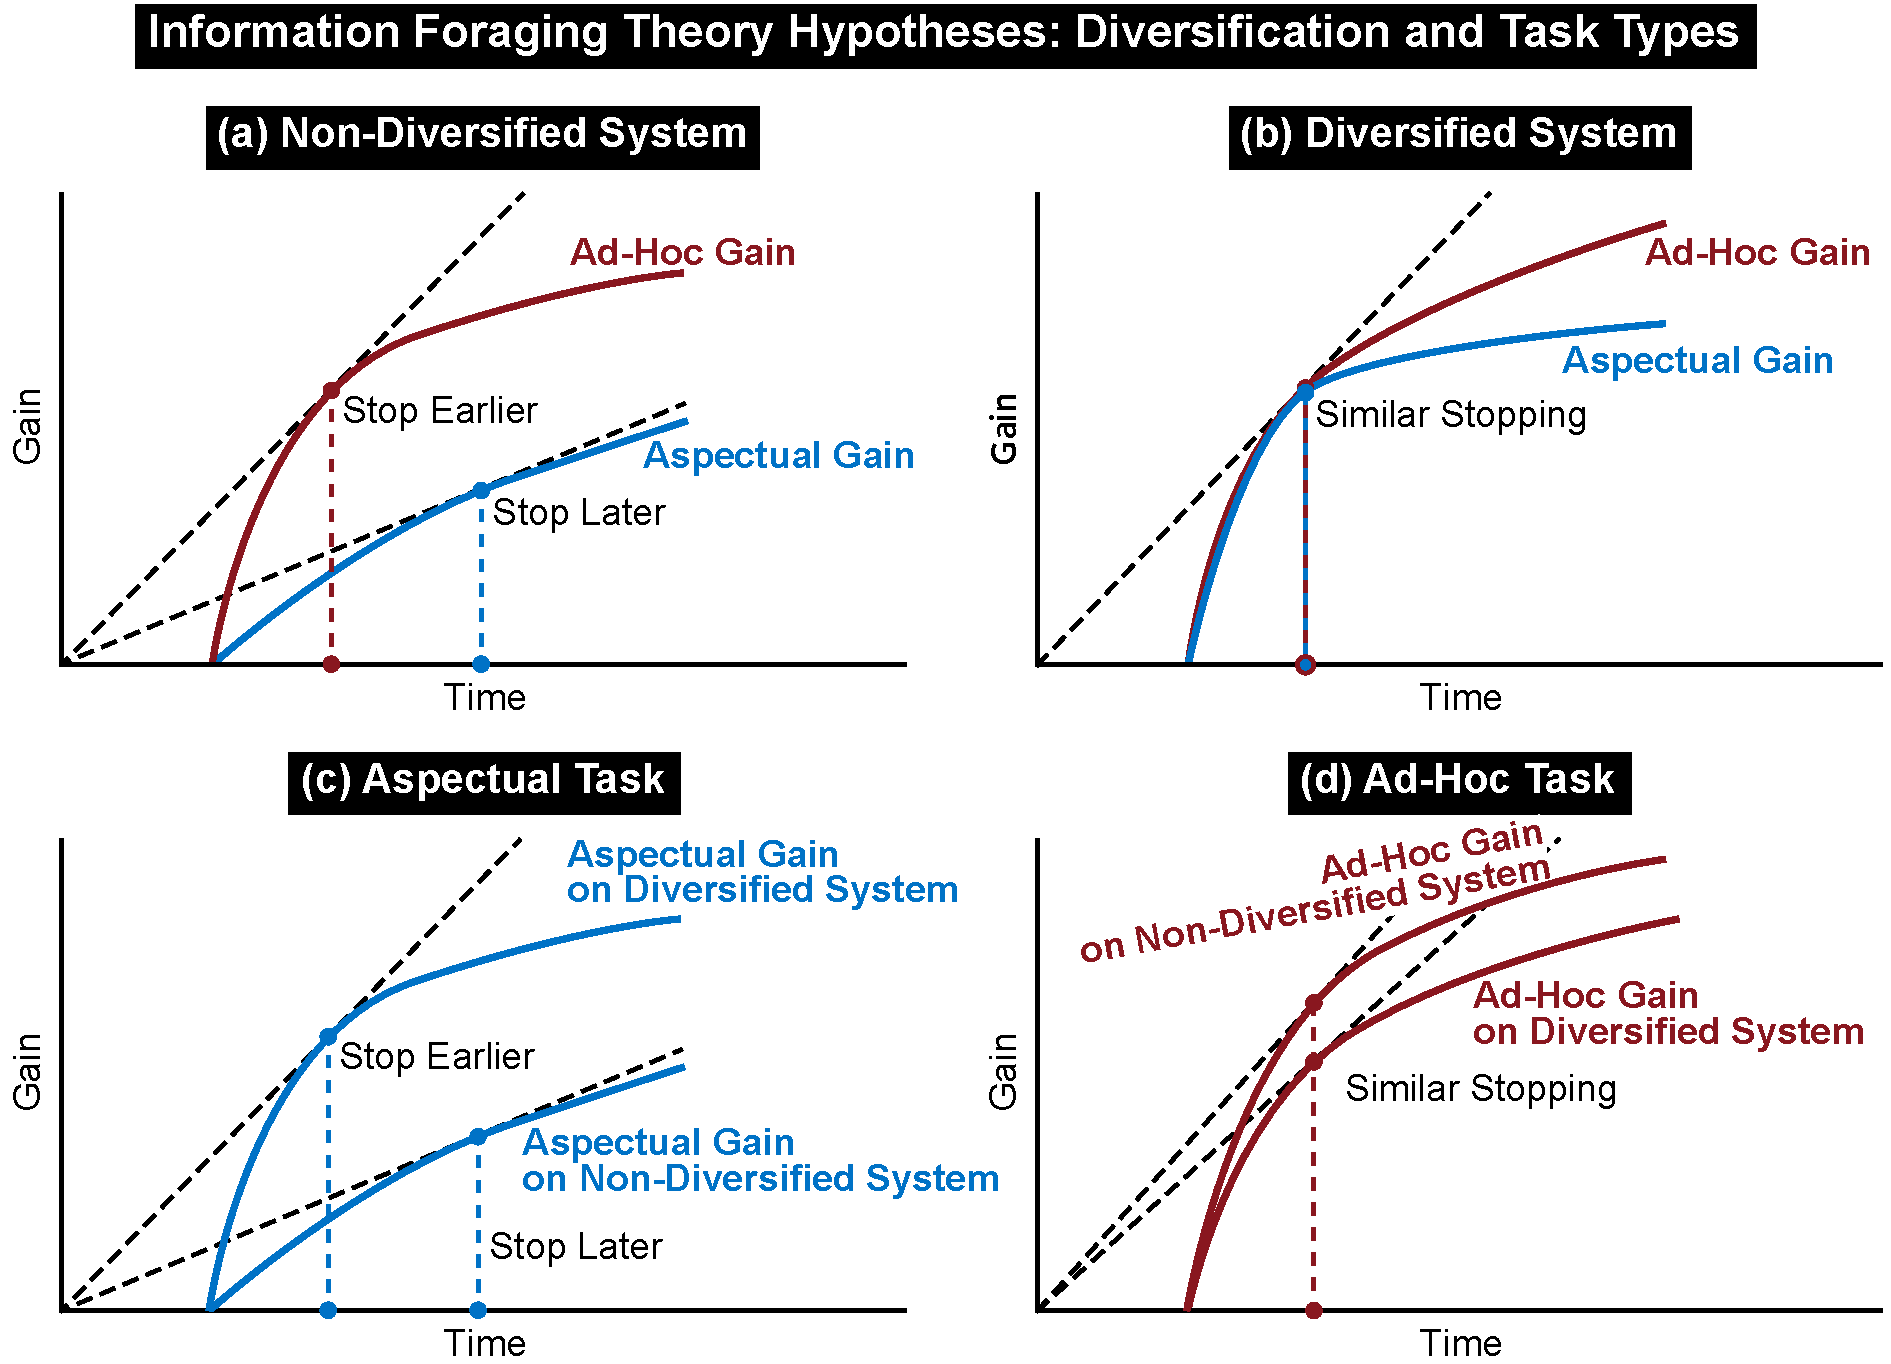
\includegraphics[width=\textwidth]{figures/ift-non-div-fromthesis.pdf}
        \vspace{-2mm}
    \caption{Information Foraging Theory: A graphical depiction of how stopping behaviour is likely to be affected on Diversified System (a), Non-Diversified System (b), Aspectual Task (c) and the Ad-Hoc Task (d).} \label{fig_ift_patches}    
    \vspace{-6mm}
\end{center}
\end{figure}


From IFT, the optimal stopping point would be different between the two tasks. Graphically we can find this point by drawing a line from the origin to the tangent of the gain curve -- the red and blue dots indicating the optimal stopping points for ad-hoc and aspectual retrieval, respectively. Thus, IFT suggests that on the non-diversified system users will examine more documents per query for the aspectual retrieval tasks when compared to the ad-hoc tasks.

In Figure~\ref{fig_ift_patches} (b), where a diversified system is being used, the gain curves for ad-hoc and aspectual retrieval will be similar -- as relevant but different documents are surfaced earlier. In the case of ad hoc topic search, these relevant (even if different) documents will still contribute to the overall gain. And in the case of aspectual retrieval, the relevant and different documents will also contribute to the overall gain -- up to the point where the documents are similar to the previously retrieved material. So IFT seems to suggest that similar stopping behaviours would be observed when searchers use the diversified system. 

Figure~\ref{fig_ift_patches} (c) shows the predicted stopping behaviour for the aspectual task, where we have plotted the aspectual gain curves from the system plots above. Interestingly, IFT suggests that searchers will stop sooner when using the diversified system, and so, if searching for the same amount of time, searchers would thus issue more queries. Finally, Figure~\ref{fig_ift_patches} (d) shows the predicted stopping behaviour for the ad hoc task, where again we have plotted the respective gain curves on each system. Note that the gain curve on the diversity may be a little lower as some irrelevant, but different material may be bubbled up - but as can be seen, we expect little difference between systems, and so the gains, and behaviour, we hypothesise will be approximately the same. Consequently, IFT suggests that there will be little difference regarding stopping behaviours between the systems on the ad-hoc retrieval tasks.

However, we found Information Foraging Theory to go counter to our intuitions on how users will behave. 
When using a standard, non-diversified system, our intuition suggests that since the aspectual retrieval task is rather exploratory, then searchers are more likely to issue more queries as they learn about the topic and try to explore efforts made by different countries to protect different species. In ~\cite{kelly2015search_tasks}, more complex search tasks are shown to require more queries. And if a searcher submits a query that retrieves relevant material such as \texttt{`protecting Pandas in China'}, then we would expect them to only select a one or two examples rather than many. In the case of ad hoc topic search, though, we would \emph{intuitively} expect that they would issue fewer queries, and examine more documents - because they don't need to find multiple aspects. However, when using a diversified system, which tries to promote different aspects of the topic, then we would \emph{intuitively} expect that searchers behaviour would change - such that when undertaking aspectual retrieval, they would issue fewer queries, and examine more documents per query. 

\subsection{Research Questions and Hypotheses} \label{sec:questions}
The primary research question of this study is: {\it how does diversification affect the search performance and search behaviour of people when performing ad hoc topic and aspectual retrieval tasks?} Based on the theoretical analysis above using IFT, we can formulate the specific following hypotheses regarding performance and behaviour:

\begin{itemize}
\item on aspectual retrieval tasks, diversification will lead to:
\begin{description}
\item [H1] fewer documents examined per query, and
\item [H2a] more queries issued, or
\item [H2b] a decrease in task completion time.
\end{description}

\item on ad hoc retrieval tasks, diversification will lead to:
\begin{description}
\item [H3] no difference in the documents examined, and
\item [H4] no difference in the number of queries issued.
\end{description}
\end{itemize}

However, the contradiction between IFT and our intuitions also provides an ulterior hypothesis. Also, given the findings from~\cite{syed2017sal}, we also hypothesise that diversification will lead to a greater awareness of the topic, regardless of the task, and so more aspects will be encountered and found.




%Under IFT, it is assumed that the forager is rational in that (i) they will visit the patch with the highest yield first, and (ii) they wish to maximize their gain per unit of time. To instantiate the model a gain function parameterized by time, i.e., $g(t)$ is required. The point where a forager should move to the next patch is when the maximum gain per unit of time is achieved. This depends on the time it takes to get to a patch, the cost of processing documents, and the distribution of relevant information (as specified by the gain function). 


